\documentclass[]{usiinfbachelorproject}


%Packages
\captionsetup{labelfont={bf}}
\usepackage[]{pdfpages}



%opening
\title{Spectrally Accurate Resampling of High Quality Rotated Images}
\author{Dylan Reid Ramelli}



\versiondate{\today}

\begin{committee}
	\advisor[Universit\`a della Svizzera Italiana, Switzerland]{Prof}{Rolf}{Krause}
	\assistant[Universit\`a della Svizzera Italiana, Switzerland]{Dr}{Patrick}{Zulian}
	\assistant[Universit\`a della Svizzera Italiana, Switzerland]{Dr}{Diego}{Rossinelli}
\end{committee}

\abstract {
	
}

\begin{document}
	
	\maketitle	
	\section{Introduction, Motivation}\label{introduction}
	For many years the amount of digital imaging data has been increasing exponentially (citation) and as such the need for acquiring this large data and process it with care has become a central point of focus. The goal of this project is to process high quality signals, in this case images, by rotating them using techniques such as the Fourier Transform, Shift Theorem, FIR filtering and CUDA parallel processing.
		
		
	WHY, WHAt for? See applications:
	
	The accurate rotation of images is very useful in applications such as Data Augmentation for Convoluted Neural Networks where one might have to rotate an image multiple times at random before feeding it to the neural network, such as in Data Visualization for multi-modal imaging. In this case we can either acquire images at different times and then combine them together so that we can manipulate the images by rotation for example to align them correctly.
	
	In our project we will use a method of rotation which was described in the article titled "Convolution-based inteprolation for fast, high-quality rotation of images"\cite{main_article} where the rotation matrix
	\begin{equation*}
		R(\theta) = 
		\begin{pmatrix}
			cos\theta & -sin\theta\\
			sin\theta & cos\theta
		\end{pmatrix}
	\end{equation*} 
	is refactorized as three matrices each of which represents a shearing in a cardinal direction.
		\begin{equation*}
		R(\theta) = 
		\begin{pmatrix}
			cos\theta & -sin\theta\\
			sin\theta & cos\theta
		\end{pmatrix}
		=
		\begin{pmatrix}
			1 & -tan\theta/2\\
			0 & 1
		\end{pmatrix}
		\cdot
		\begin{pmatrix}
			1 & 0\\
			sin\theta & 1
		\end{pmatrix}
		\cdot
		\begin{pmatrix}
			1 & -tan\theta/2\\
			0 & 1
		\end{pmatrix}
	\end{equation*} 
	
	The first matrix shears the image in the $x$ direction by $\Delta_x = -y\cdot tan(\theta/2)$, the second matrix shears the image in the $y$ direction by $\Delta_y = x \cdot sin(\theta)$ and the last matrix shears again in the $x$ direction by $\Delta_x$.\\
	
	Given this definition of a 2D rotation we can perform the operation as a sequence of three 1D translations on the 1D input array that represents our image.
	
	"Explain 2D to 3D."
	
	FT: Direct solver instead of iterative, takes in a lot of data.
	
	
	\section{State of the art}
	For certain applications such as... it is required to be able to rotate images while maintaining the highest quality possible. To achieve satisfying results the general approach is to use bilinear and nearest neighbour interpolation.
	
	
	Include images from Diego of blood vessels in the heart iI think
	
	
	\iffalse
	
	\subsection{Interpolation}
	Sampled version of our translated signal is:
	\begin{equation}
		(T_\Delta s)[k] = \sum_{l \in Z}^{} c(l)\varphi(k - \Delta - l)
	\end{equation}
	Where $\varphi$ is our generating function.
	\subsubsection{Linear Interpolation}
	With linear interpolation we want to estimate the coordinates of a point from a given number of samples. 
	
	Linear interpolation model of function sin(x) with $N = 2$:
	\begin{equation}
		\beta^1(x) = 
		\begin{cases}
			1 - |x|, & |x| < 1    \\
			0,       & otherwise, 
		\end{cases}
	\end{equation}
	\begin{center}
		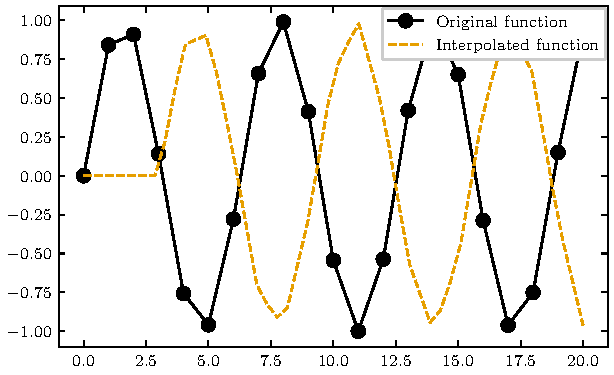
\includegraphics{"images/linear_interpolation_example.pdf"}
	\end{center}
	
	Cubic spline interpolation model of function sin(x) with $N=4$:
	\begin{equation}
		\beta^3(x) = 
		\begin{cases}
			2/3 - |x|^2 + |x|^3/2, & 0 \leq|x| < 1  \\
			(2-|x|)^3/6,           & 1 \leq |x| < 2 \\
			0,                     & 2 \leq |x|     
		\end{cases}
	\end{equation} \cite{main_article}
	
	\begin{center}
		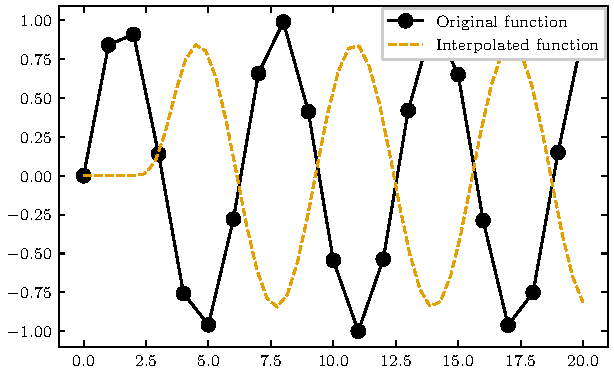
\includegraphics{"images/cubic_interpolation_example.pdf"}
	\end{center}
	
	Standard 2-D interpolation formula for computing the value of the image at location $(x,y)$
	\begin{equation}
		s(x,y) = \sum_{k = k_0}^{k_0+L-1}\sum_{l=l_0}^{l_0+L-1} c(k,l)\varphi(x-k)\varphi(y-l)
	\end{equation}
	
	\fi
	

	\section{Project Requirements}
	To complete this project I made use of different tools such as, Python, Jupyter Notebook, C/C++ and CUDA.
	
	
	
	\subsection{Frequencies of a signal}
	\begin{equation}
		freq_{n} = \lfloor \frac{n}{2} \rfloor + 1
	\end{equation}
	Visual representation with $n=3$ of the discrete Fourier transform of a function $g(x)$
	
	\begin{equation*}
		G_m = \displaystyle\sum_{k=0}^{N-1}g(k)e^{-i \frac{2\pi}{N}km}
	\end{equation*}
	
	To shift a signal by a fractional amount it is imperative to use the correct frequency when doing so.
	
	Given that for $n$ samples we have $\lfloor \frac{n}{2} \rfloor + 1$ distinct frequencies
	
	
	\begin{figure}
		\centering
		\include{file}
		\caption{Unit circle with N = 3, }
	\end{figure}
	
	Euler's Formula
	\begin{equation}
		e^{ix} = cos(x)  + i sin(x)
	\end{equation}
	
	Useful property:
	\begin{equation}
		cos(w)= \frac{1}{2}(e^{iw}+ e^{-iw})
	\end{equation}
	
	
	\subsection{Fourier Transform with Shift Theorem}
	Here we derive the shift theorem for a discrete signal starting from the normal Fourier Transform with $g_k$ being our 1D input array, $N$ the number of samples and $m$ the frequency:
	\begin{equation*}
		G_m = \displaystyle\sum_{k=0}^{N-1}g_k[k]e^{-i \frac{2\pi}{N} km}
	\end{equation*}
	
	Now instead of $g_k[k]$, we want $g_k[k - \delta]$ where $\delta$ is the amount we want to shift.
	So the above equation can be rewritten as:
	\begin{equation*}
		Z_m = \displaystyle\sum_{k=0}^{N-1}g_k[k - \delta]e^{-i \frac{2\pi}{N} km}
	\end{equation*}
	
	\begin{equation*}
		Z_m = \displaystyle\sum_{r = 0 - \delta}^{N-1-\delta}g_k[r]e^{-i \frac{2\pi}{N} km}, r = k - \delta 
	\end{equation*}
	
	Since $r = k - \delta$ then $ k = r + \delta$, and as such:
	
	\begin{equation*}
		Z_m = \displaystyle\sum_{r= -\delta}^{N-1 - \delta}g_k[r]e^{-i \frac{2\pi}{N} (r + \delta)m}
	\end{equation*}
	
	We can then separate the exponential:
	
	\begin{equation*}
		Z_m = \displaystyle\sum_{r= -\delta}^{N-1 - \delta}g_k[r]e^{-i \frac{2\pi}{N} rm}e^{-i \frac{2\pi}{N}  \delta m}
	\end{equation*}
	
	And factor it out of the sum:
	
	\begin{equation*}
		Z_m = e^{-i \frac{2\pi}{N}  \delta m} \displaystyle\sum_{r= -\delta}^{N-1 - \delta}g_k[r]e^{-i \frac{2\pi}{N} rm}
	\end{equation*}
	
	The sum now has exactly the same as before:
	
	\begin{equation*}
		Z_m = e^{-i \frac{2\pi}{N}  \delta m} \displaystyle\sum_{k=0}^{N-1}g_k[k]e^{-i \frac{2\pi}{N} km}
	\end{equation*}
	
	\begin{equation}
		Z_m = e^{-i \frac{2\pi}{N}  \delta m} G_m = H_m \cdot G_m
	\end{equation}
	
	
	Here is a small example made in python:
	
	\begin{figure}[h]
		\centering
		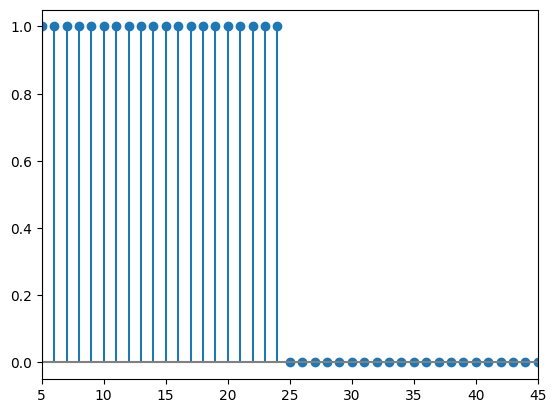
\includegraphics[width=0.5\columnwidth]{images/box_original_n50.png}
		\caption{Original 1D function.}
	\end{figure}
	
	\begin{figure}[h]
		\centering
		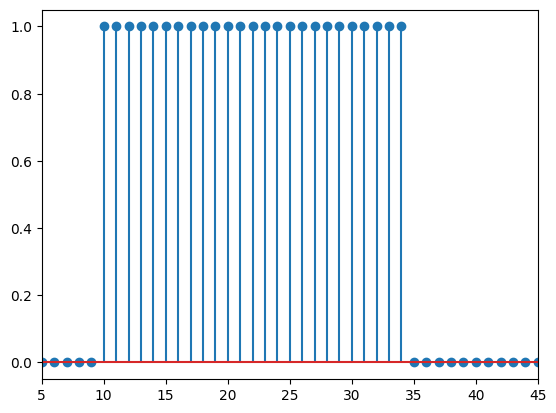
\includegraphics[width=0.5\columnwidth]{images/box_shifted_delta10_n50.png}
		\caption{Function shifted by $\delta=10$}
	\end{figure}
	
	
	The above equation works well for non fractional shifts but has a certain problem when we want to shift by a fractional amount.
	"Explain why".\\
	To solve this we need to take into consideration the negative frequencies and in particular if the number of samples is odd or even.
	Normally we multiply each sample by its corresponding phase, which is based on the frequency number $m$
	but since we need to take into consideration the negative frequencies we can define a function called wavenum that returns the correct frequency index to use in the phase shift:
	\begin{equation*}
		wave\_n(m) = (m + N // 2) \bmod N - (N//2)
	\end{equation*}
	
	\begin{figure}[h]
		\centering
		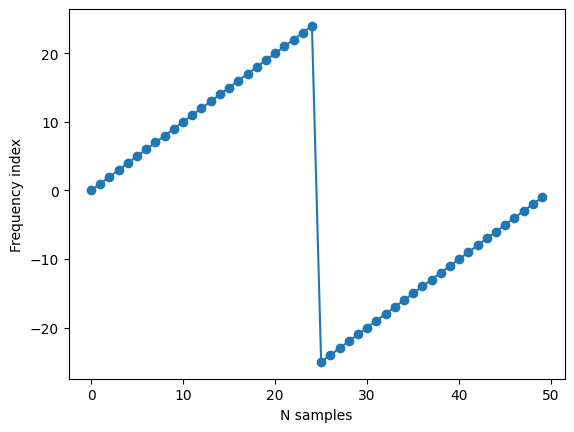
\includegraphics[width=0.5\columnwidth]{images/wavenum_n50.png}
		\caption{Wavenum function with $N=50$}
	\end{figure}
	
	\begin{equation*}
		H_m = e^{-i \frac{2\pi}{N}  \delta wave\_n(m)}
	\end{equation*}
	
	\begin{equation}
		Z_m = H_{wave\_n(m)} \cdot G_m
	\end{equation}	
	
	

	
	\begin{figure}[h]
		\centering
		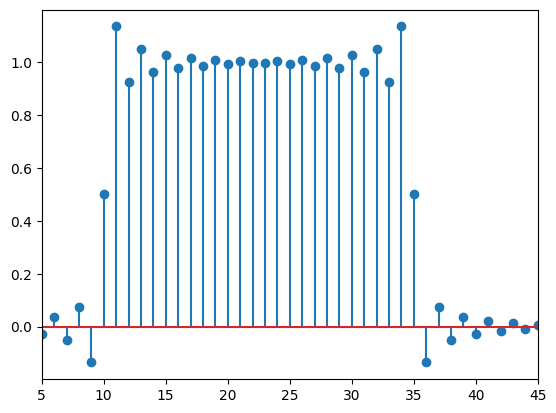
\includegraphics[width=0.5\columnwidth]{images/box_shifted_delta10_1_n50.png}
		\caption{Shifted function by $\delta=10.5$}
	\end{figure}
	
	
	\subsection{Lanczos Filter and FIR}
	To alleviate the problems that arise when shifting a signal by a fractional amount we can use a filter $L$ that is convoluted with the shifted signal.
	
	\begin{equation*}
		L_m = \frac{sin(a)}{a} |_{a = sin(\frac{2\pi wave\_n(m)}{N})}
	\end{equation*}
	
	Apply lanczos filter to fractional shift to smooth the result.
	
	\begin{equation*}
		Z_m = L_m \cdot H_m \cdot G_m
	\end{equation*}
	\begin{figure}[h]
		\centering
		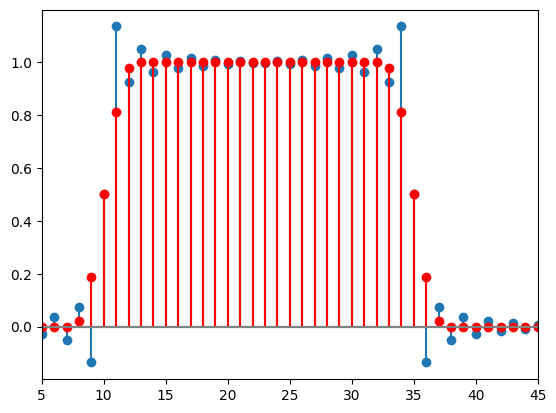
\includegraphics[width=0.5\columnwidth]{images/box_shifted_lanczos_delta10_1_n50.png}
		\caption{Shifted function by $\delta=10.5$ with lanczos filter applied (red), no filter(blue).}
	\end{figure}
	
	
	\newpage
	
	\section{Project Design}
	Explain 1D,2D,3D transposition.
	Simplification of 2D rotation using 1D translations.
	
	
	
	\section{Implementation}
	\begin{itemize}
		\item Problems while implementing the code
		\item Indexing frequencies...
		\item practical problems...
	\end{itemize}
	
	\section{Result}
	
	
	\begin{itemize}
		\item Rotate image many times like in the paper
		\item look for artefacts
		\item compare with C code gathernoloss.c
		\item quality, quantity
	\end{itemize}
	
	
	\section{Solution}
	\section{Validation}
	\section{Conclusion}
	\begin{itemize}
		\item Summary
		\item limitations
	\end{itemize}
	\bibliographystyle{plain}
	\bibliography{references}
	
\end{document}